\documentclass[11pt]{article}

\usepackage[margin=1in]{geometry}
\usepackage{amsmath,amssymb}
\usepackage{booktabs}
\usepackage{graphicx}
\usepackage{hyperref}
\usepackage{microtype}

\newcommand{\UM}{U_{\mathrm{M}}}
\newcommand{\Usc}{U_{\mathrm{sc}}}
\newcommand{\Urel}{U_{\mathrm{rel}}}
\newcommand{\BSBM}{B_{\mathrm{S}}/B_{\mathrm{M}}}
\newcommand{\code}[1]{\texttt{#1}}

\title{Clean-Room Reconstruction and Physical-Consistency Audit of the\\
Halekas et al. (2008) Lunar-Potential Example}
\author{ESPG Lunar Potential Map Project}
\date{11 July 2026}

\begin{document}
\maketitle

\begin{abstract}
We perform a four-phase clean-room reconstruction of the Halekas et al. (2008)
Lunar Prospector Electron Reflectometer (LP ER) surface-potential example near
14:45 UT on 29 April 1999.  A literal public reconstruction initially obtains
$\Urel=-261$~V rather than the published $-171$~V.  Integrating a sharp physical
boundary over actual angular support and applying the documented fractional
energy response moves the joint estimate to $-161$~V under two normalization
orders.  Removing the beam-amplitude rail and fitting the measured broad beam
gives a stable beam-only scale near $-145$~V and joint estimates of
$-151$ to $-161$~V, but boundary-only estimates remain strongly dependent on
cone refilling, broadening, masking, and magnetic ratio.  A direct Figure~5
raster comparison then favors spectrum 654 over the previously assumed 653;
its beam amplitude matches the publication, but its extracted loss-cone
boundary does not independently select the published $(\Urel,\BSBM)$ pair.
Publication-like boundary voltages appear when $\BSBM=0.975$ is imposed, while
free fits prefer substantially different field ratios.  We conclude that the
upward secondary beam robustly establishes a negative spacecraft-relative
voltage scale of order 145--160~V in the benchmark interval.  The public data
and reconstructed method do not provide a stable independent two-parameter
loss-cone confirmation of the exact published $-171$~V, 0.975 pair.
\end{abstract}

\section{Purpose and Epistemic Status}

The purpose of this experiment is not to tune a modern estimator until it
matches a published number.  It is to distinguish four questions:
\begin{enumerate}
  \item Can the public description reproduce the historical result?
  \item Which instrument and representation choices control reproduction?
  \item Do the beam and loss-cone boundary independently support one voltage?
  \item Does the archived Figure~5 distribution uniquely support the published
        voltage and magnetic ratio?
\end{enumerate}
The published value is a historical reference, not ground truth.  Stable
disagreement may indicate a missing private processing detail, different manual
quality control, or bias in the published point estimate.

The evidentiary basis is frozen in
\code{provenance/halekas-cleanroom-reconstruction.md}, with a SHA-256 checksum.
Phase A4 additionally freezes the native embedded Figure~5 data raster and its
color-calibrated value map.  Publicly unresolved choices are represented as
explicit branches rather than silently selected defaults.

\section{Data and Physical Observables}

The LP ER three-dimensional product contains 15 sequential energy rows and 88
look directions.  The benchmark neighborhood consists of spectra 652--654.
The publication reports
\begin{equation}
  \Usc=+11~\mathrm{V},\qquad
  \UM=-160~\mathrm{V},\qquad
  \Urel=\UM-\Usc=-171~\mathrm{V},\qquad
  \BSBM=0.975.
\end{equation}

The adiabatic boundary equation is
\begin{equation}
  \sin^2\alpha_c(E)=\BSBM
  \left(1+\frac{\UM}{E-\Usc}\right),
  \label{eq:boundary}
\end{equation}
where the reflected-side boundary plotted at high pitch is
$\beta(E)=180^\circ-\alpha_c(E)$.  The upward secondary beam is centered at
\begin{equation}
  E_{\mathrm{beam}}=\Usc-\UM=-\Urel
\end{equation}
in electron-volt/volt numerical units when the beam reaches the spacecraft.

The measured quantity is a normalized reflected-to-incident distribution.
Two public-evidence normalizations remain plausible: division by a conjugate
incident direction and division by the incident-hemisphere mean.  The 2008
method minimizes an unweighted squared difference of logarithmic normalized
fluxes over the complete distribution.  This objective is descriptive; it has
no recovered variance scale and its differences are not confidence levels.

\section{Phase A1: Literal Public Reconstruction}

Phase A1 rebins the 88 sectors into 16 fixed 11.25-degree pitch bins, uses a
hard loss-cone boundary, tests cone floors 0.05 and 0.10, and represents the
beam by one energy row and two field-aligned pitch bins.  Beam amplitude is
either fixed from the measured excess or profiled on a nuisance grid.  Eight
branches cross normalization, floor, and amplitude handling.

All branches select
\begin{equation}
  \UM=-250~\mathrm{V},\qquad
  \Urel=-261~\mathrm{V},\qquad
  \BSBM=0.910.
\end{equation}
The result is stable but fails the predeclared 25~V historical voltage gate.
The measured beam occupies both the 113 and 196~eV rows, while the synthetic
beam is assigned to only one.  The measured loss-cone transition is graded but
the model is binary.  Phase A1 therefore diagnoses a representation failure,
not evidence for a physically exact $-261$~V potential.

\begin{figure}[ht]
  \centering
  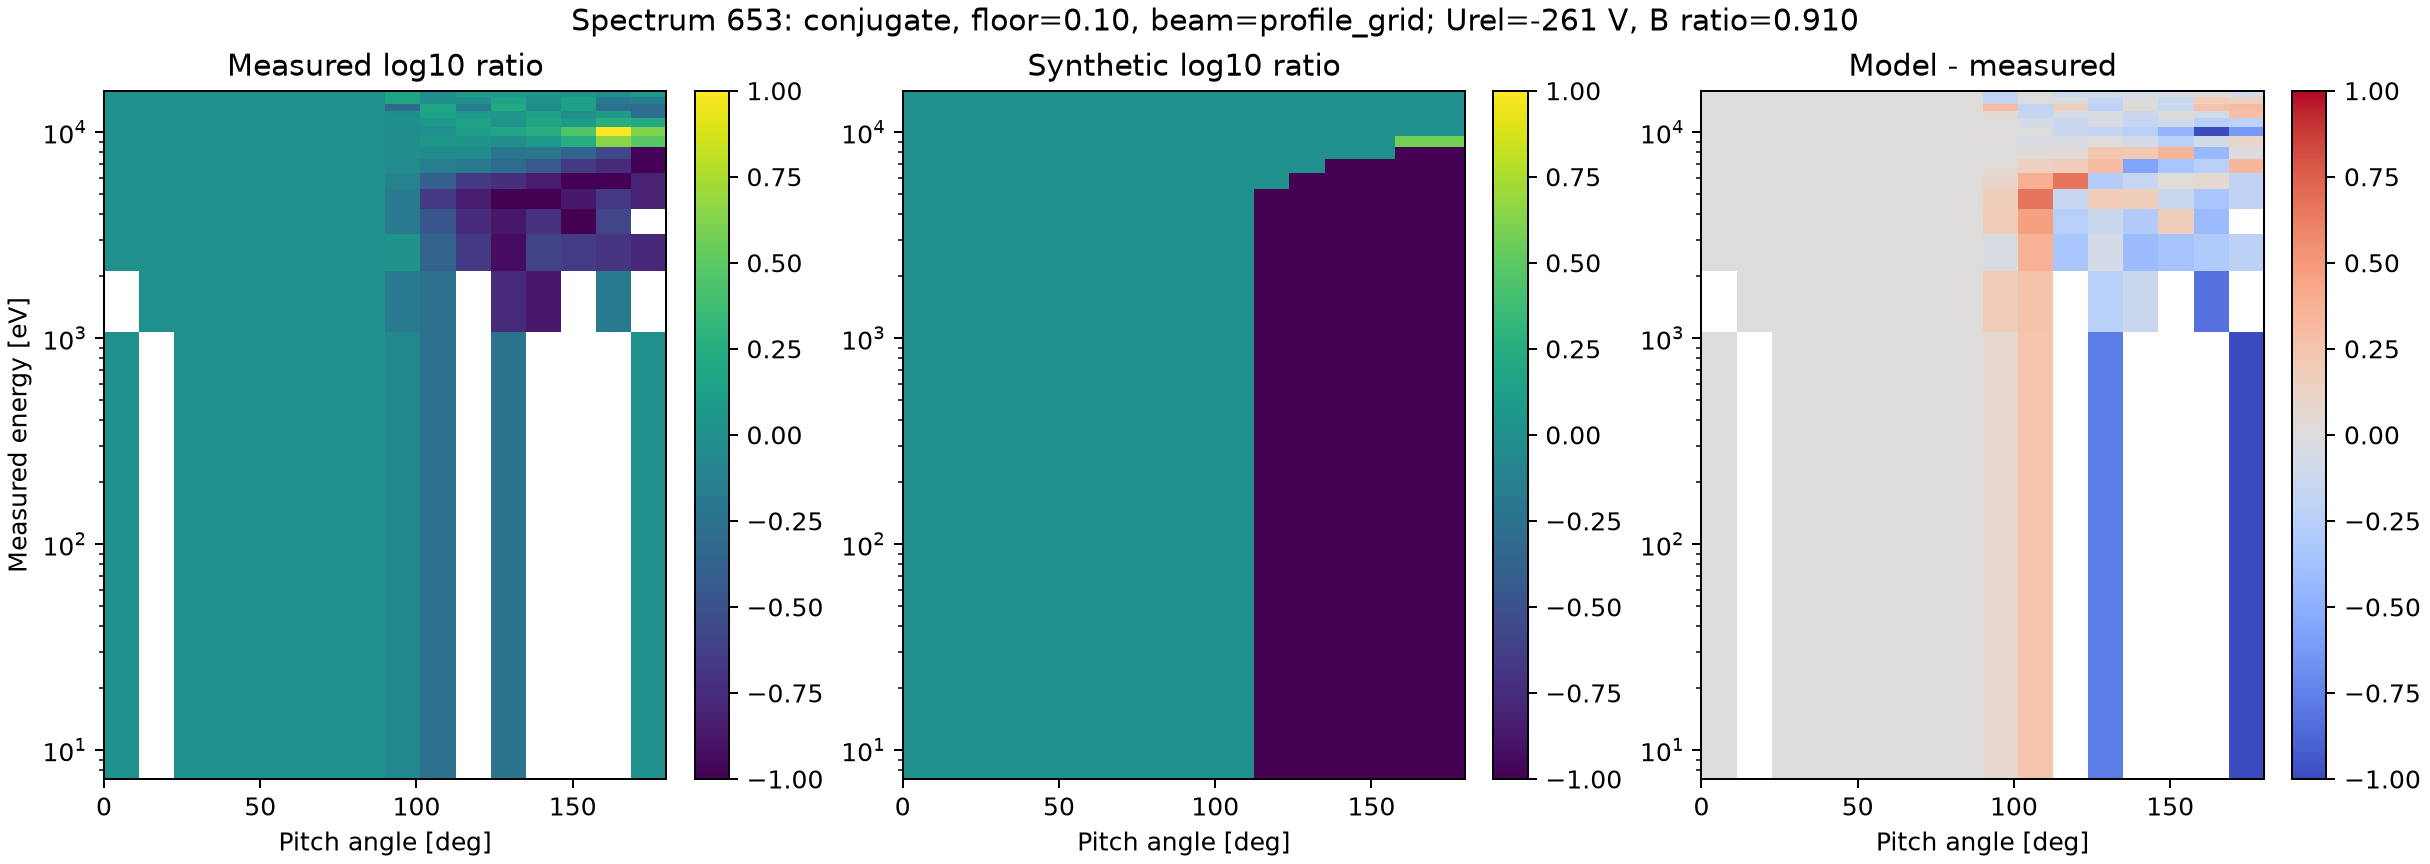
\includegraphics[width=\textwidth]{../phase_a_comparison.png}
  \caption{Phase A1 measured, synthetic, and residual distributions for the
  lowest-objective literal branch.}
  \label{fig:a1}
\end{figure}

\section{Phase A2: Instrument Representation}

Phase A2 freezes a $2\times2\times2$ comparison:
\begin{itemize}
  \item bin flux then divide versus divide native sector pairs then bin;
  \item evaluate the sharp boundary at the pitch-bin center versus average the
        sharp sector-level model over the sectors that contributed to the bin;
  \item assign the beam to the nearest energy row versus apply a Gaussian
        response with $\mathrm{FWHM}/E=0.48$.
\end{itemize}
The cone floor is 0.10 and beam amplitude is profiled on $[0,8]$.

Nearest-row branches remain at $\Urel=-251$ to $-261$~V.  The two
support-integrated fractional-response branches agree exactly despite reversing
normalization order:
\begin{equation}
  \Urel=-161~\mathrm{V},\qquad \BSBM=0.880,
\end{equation}
only 10~V from the historical voltage.  Thus the initial discrepancy is
primarily a discretized beam-response artifact, with angular support integration
required for representation stability.  No arbitrary sigmoid is needed to
recover the historical voltage scale.

However, both publication-like branches place beam amplitude at the frozen
upper limit of 8.  Independent fits give a beam voltage near $-145.5$~V and a
boundary-only voltage near $-281$~V.  Reproducing one joint scalar does not show
that the two observables agree.

\begin{figure}[ht]
  \centering
  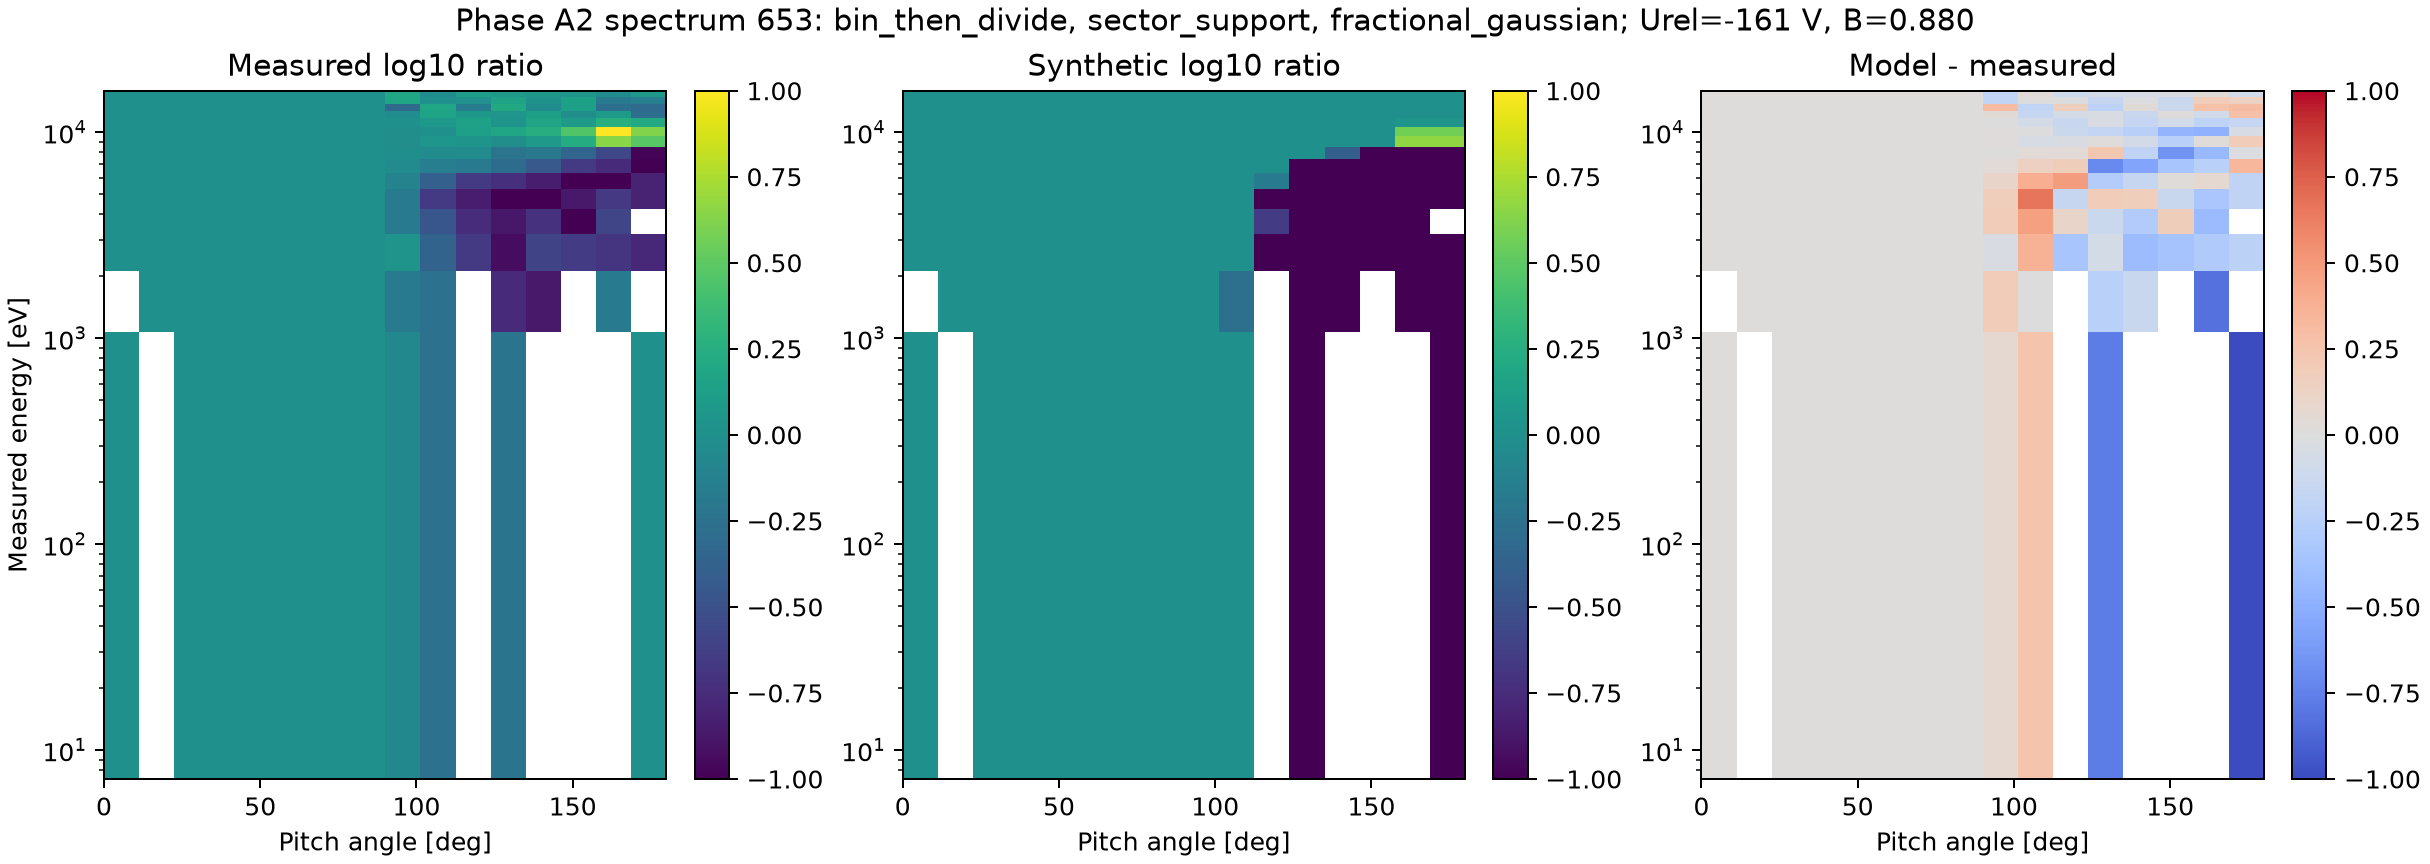
\includegraphics[width=\textwidth]{../phase_a2_comparison.png}
  \caption{Best Phase A2 support-integrated, fractional-response comparison.}
  \label{fig:a2}
\end{figure}

\section{Phase A3: Physical-Consistency Stress Test}

Phase A3 removes the artificial beam rail and crosses two normalization orders,
narrow versus broad beam pitch response, sharp versus five-degree broadened
boundary, and cone floors 0.10 versus 0.25.  Fractional energy response is held
fixed.  Beam amplitude is profiled on $[0,20]$.

All 16 joint branches return $\Urel=-151$ or $-161$~V without amplitude or
voltage rails.  The lowest descriptive objective uses a broad Gaussian beam,
five-degree boundary, and floor 0.25:
\begin{equation}
  \Urel=-151~\mathrm{V},\qquad \BSBM=1.000,
  \qquad A_b=14.0.
\end{equation}
The objective per nominal degree of freedom falls from 0.1938 in A2 to 0.1233,
although structured high-energy residuals remain.

The independent two-dimensional beam fit is highly stable across normalization:
\begin{equation}
  {\Urel}_{\mathrm{beam}}=-145.4~\mathrm{V},\qquad
  A_b\simeq12.2,\qquad
  \mathrm{FWHM}_{\alpha}\simeq58^\circ.
\end{equation}
Boundary-only results, by contrast, span $-281$~V to $+9$~V as floor,
broadening, and masking change.  The joint estimate is beam-dominated.  The
loss cone does not provide a stable independent voltage under this model family.

\begin{figure}[ht]
  \centering
  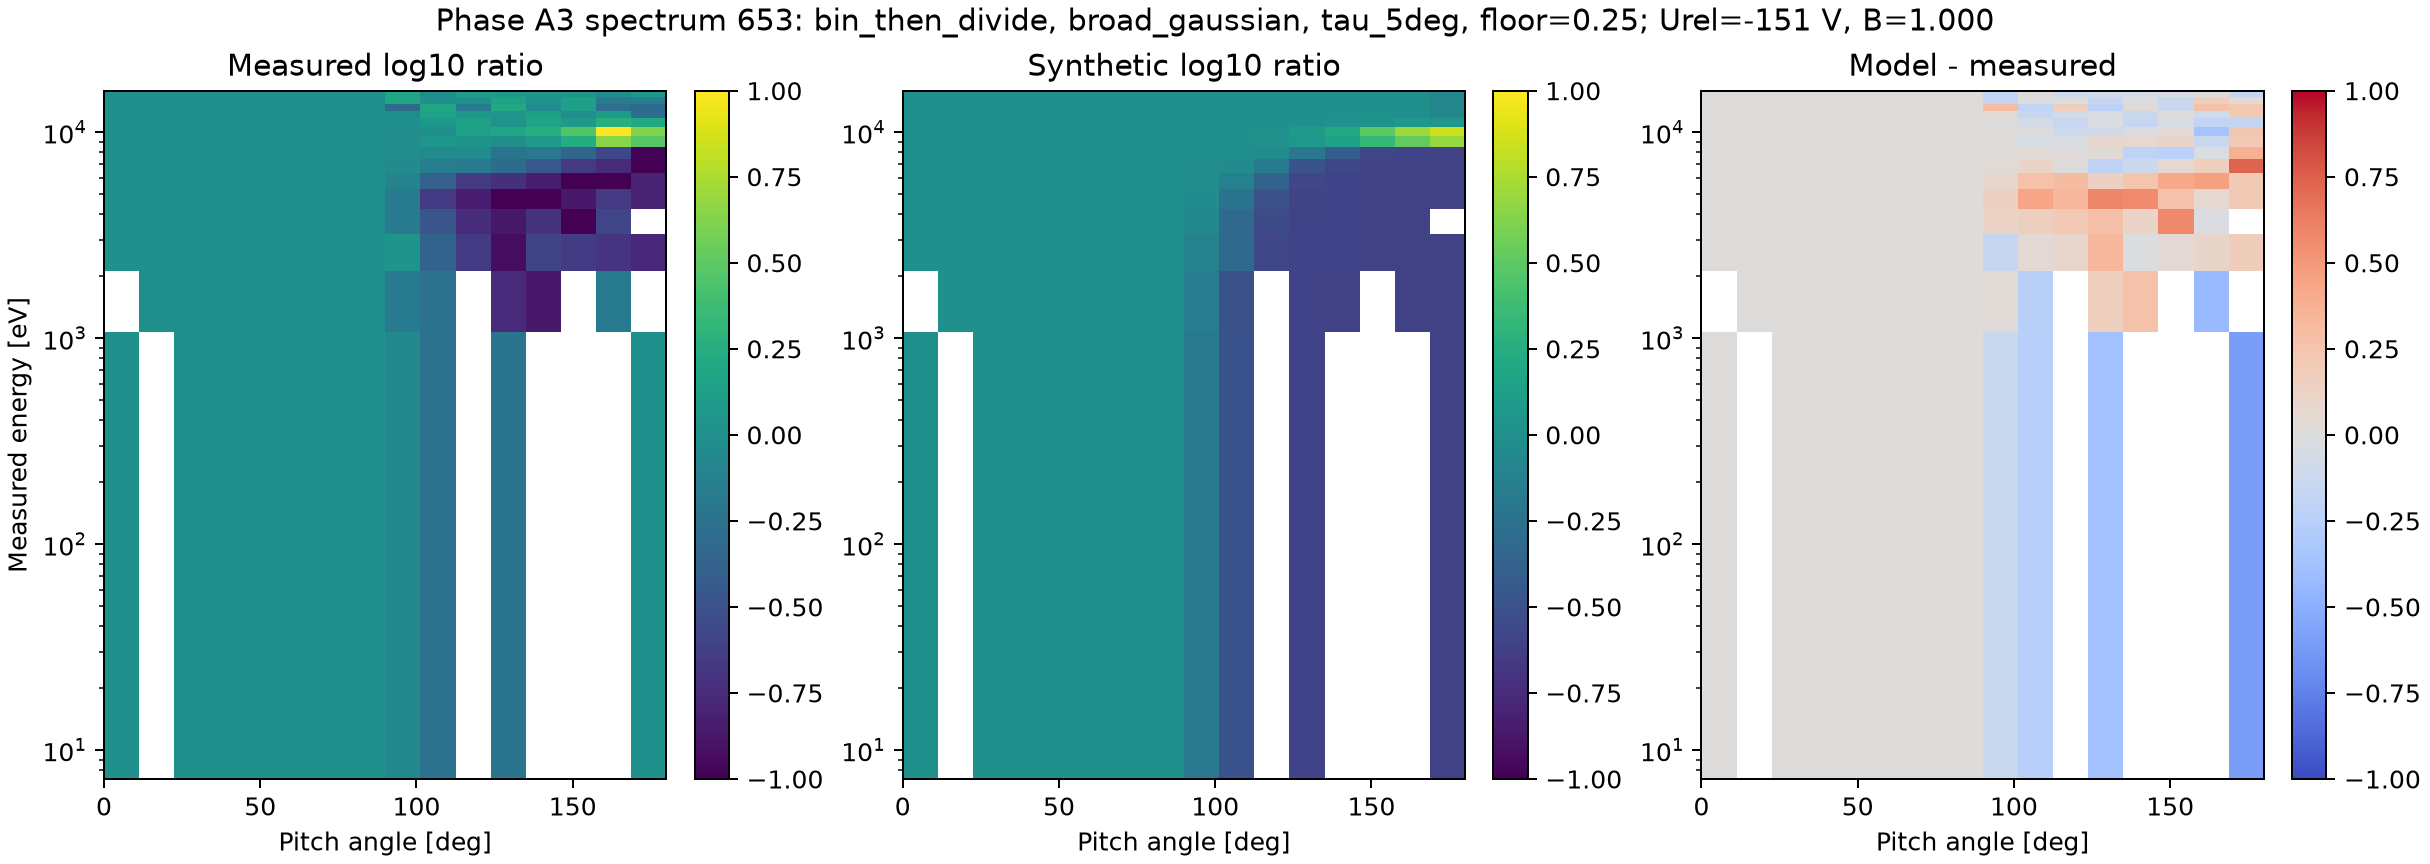
\includegraphics[width=\textwidth]{../phase_a3_comparison.png}
  \caption{Best Phase A3 model after extending beam amplitude and angular
  support.  Coherent residual structure remains despite the lower objective.}
  \label{fig:a3}
\end{figure}

\section{Phase A4: Figure Identity and Boundary-First Inference}

Phase A4 stops fitting a joint beam-plus-cone voltage.  It first compares
spectra 652--654 with the frozen Figure~5 raster, then extracts a transition at
each energy before applying equation~\eqref{eq:boundary}.

\subsection{Figure 5 identity}

The primary morphology metric is reflected-side logarithmic RMSE with no fitted
rescaling.  Table~\ref{tab:panel} gives the closest normalization per spectrum.

\begin{table}[ht]
  \centering
  \caption{Figure~5 panel-identity comparison.}
  \label{tab:panel}
  \begin{tabular}{lrrrr}
    \toprule
    Spectrum & Normalization & Log RMSE & Correlation & Beam peak \\
    \midrule
    652 & conjugate & 0.646 & 0.873 & 15.28 \\
    653 & incident mean & 0.434 & 0.915 & 10.39 \\
    654 & incident mean & \textbf{0.399} & 0.926 & \textbf{4.35} \\
    Published & -- & -- & -- & 4.48 \\
    \bottomrule
  \end{tabular}
\end{table}

Spectrum 654 begins at 14:45:28 UT and is a better panel candidate than spectrum
653 despite 653 having the closest midpoint to the rounded 14:45 label.  With
conjugate normalization, 654 has RMSE 0.417, correlation 0.932, and beam peak
4.51.  Both representations favor 654.  The match remains imperfect, so private
processing or display differences are not excluded.

\begin{figure}[ht]
  \centering
  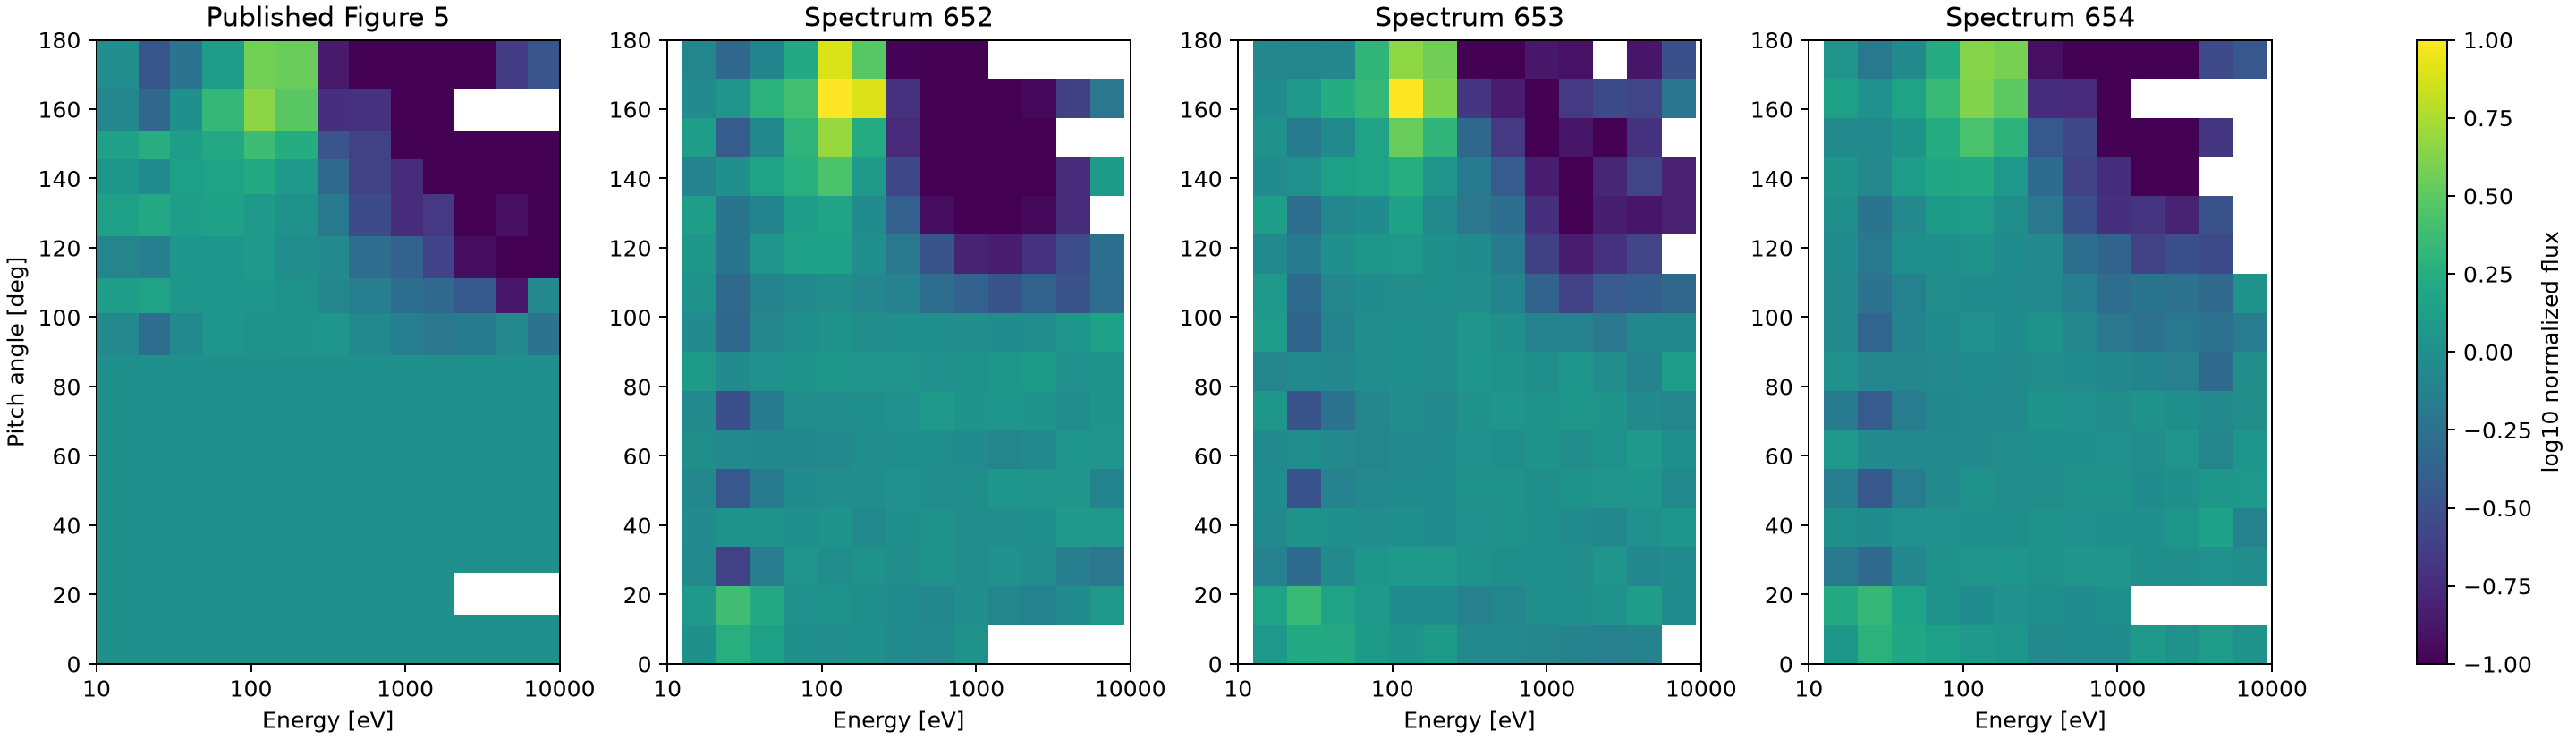
\includegraphics[width=\textwidth]{../phase_a4_panel_comparison.png}
  \caption{Frozen published Figure~5 raster and incident-mean candidates.
  Spectrum 654 most closely reproduces the beam amplitude and broad morphology.}
  \label{fig:panel}
\end{figure}

\subsection{Boundary extraction}

For each native reflected sector at 300--10000~eV, Phase A4 fits
\begin{equation}
  R(\alpha)=R_{\mathrm{in}}+\Delta R
  \left[1+\exp\left(-\frac{\beta-\alpha}{w}\right)\right]^{-1},
  \label{eq:transition}
\end{equation}
where the cone level, contrast, boundary $\beta$, and width are all free.  One
hundred deterministic sector bootstraps estimate boundary uncertainty, with a
5.625-degree resolution floor.  The extracted boundary points are then fit with
equation~\eqref{eq:boundary} under free $(\UM,\BSBM)$, fixed published
$\BSBM=0.975$, and a high-energy asymptotic field ratio.

The archived magnetic vector is exactly repeated across all 15 rows of each
spectrum.  Row-field and sweep-mean pitch calculations are identical to
$10^{-13}$ degrees.  Energy-correlated magnetic rotation is not responsible for
the observed boundary behavior.

Under preregistered acceptance, spectrum 652 shows a coherent weak-potential
trend and gives $\Urel=-41$ to $-61$~V with $\BSBM=0.975$--0.990.  Spectrum 653
is non-monotonic and gives $-111$ to $-151$~V while requiring
$\BSBM=1.005$--1.050; conjugate fits reach the upper field-ratio edge.  Spectrum
654, the closest panel, gives only $-1$ to $-41$~V when both parameters are free,
with $\BSBM=0.750$--0.825.

Several per-energy transitions hit nuisance bounds.  The preregistered results
remain primary, but a labeled strict check excludes those points.  Spectrum 652
remains near $-31$ to $-61$~V; spectrum 653 loses the low-energy points carrying
its negative voltage and moves near zero; spectrum 654 gives free fits around
$-61$ to $-81$~V with $\BSBM=0.755$--0.795.  If $\BSBM=0.975$ is imposed, strict
spectrum-654 boundaries instead imply $\Urel=-181$ to $-191$~V.  Those
fixed-ratio objectives are substantially worse than the free low-ratio fits.

\begin{figure}[ht]
  \centering
  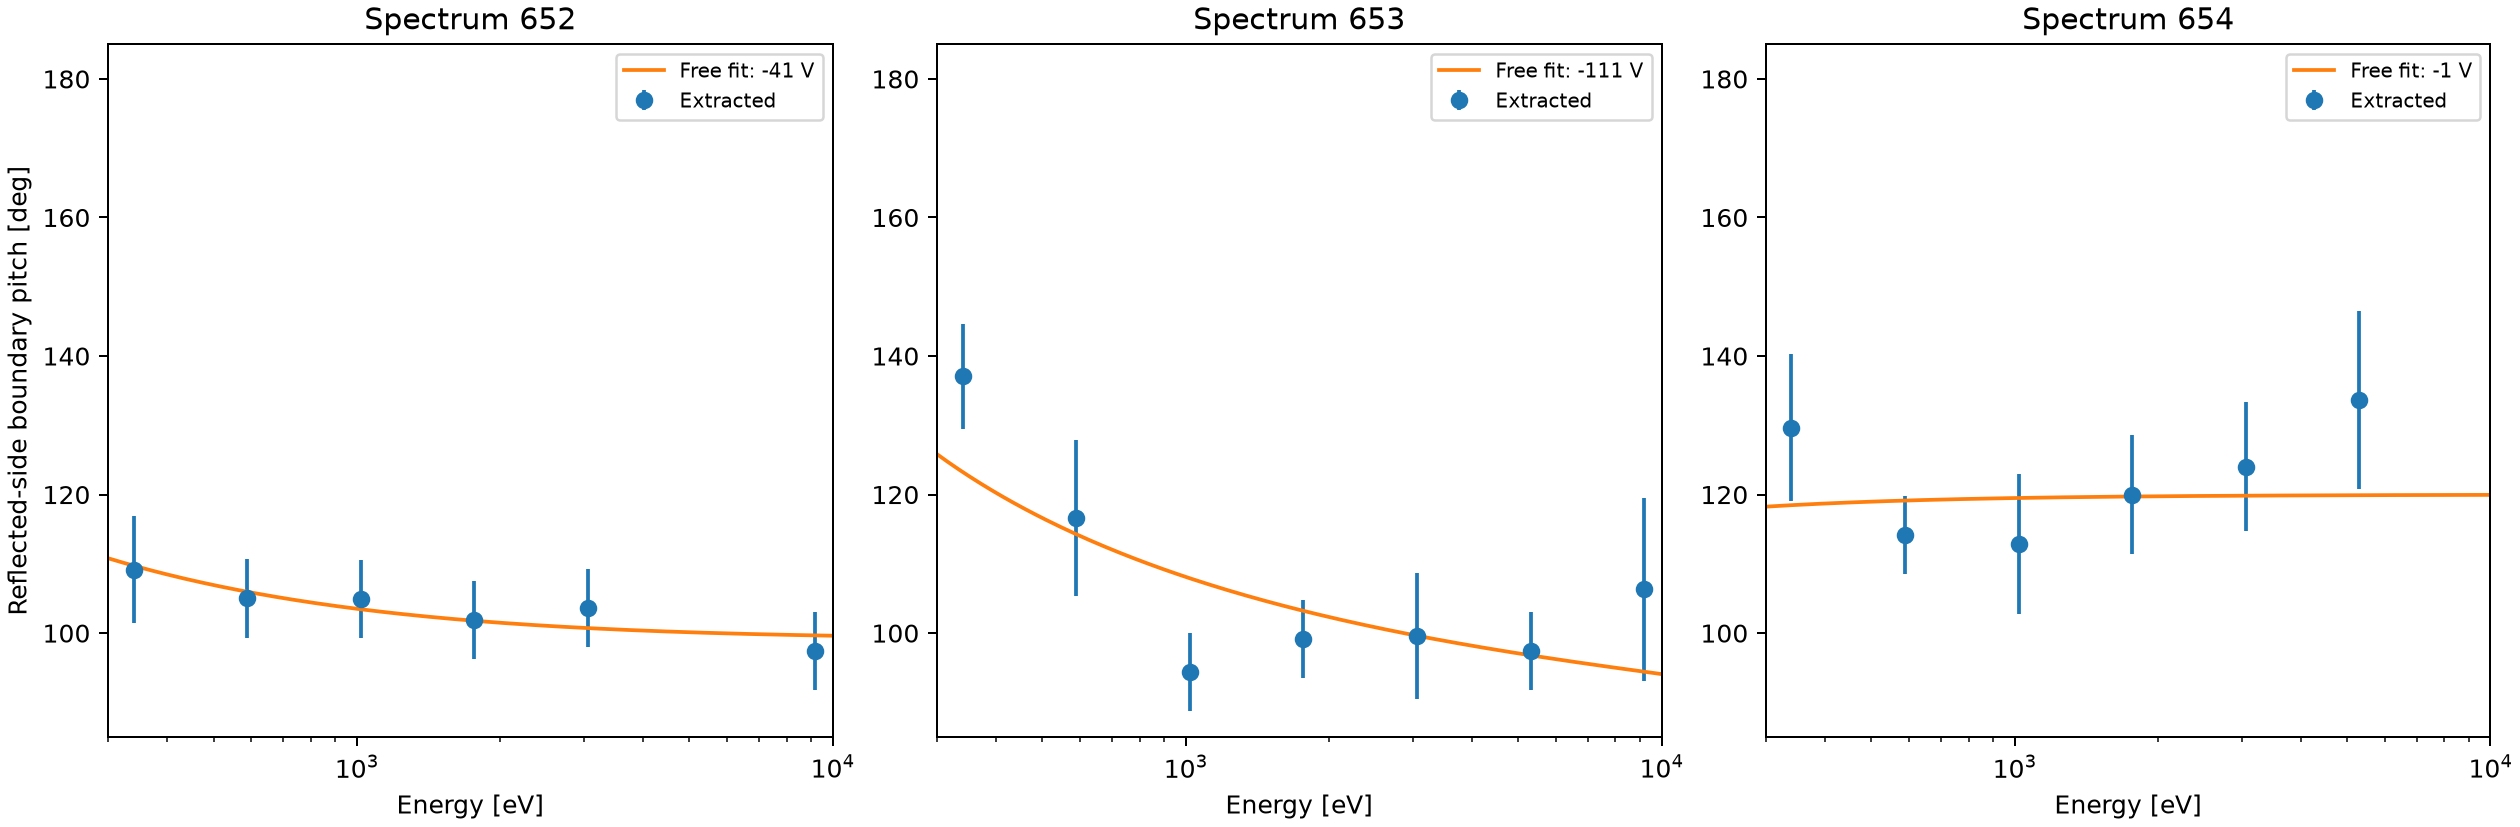
\includegraphics[width=\textwidth]{../phase_a4_boundaries.png}
  \caption{Incident-mean, equal-sector boundary points and preregistered free
  adiabatic fits.  Spectrum 652 is coherent, 653 is non-monotonic, and 654 trends
  incompatibly with a large negative free potential.}
  \label{fig:boundaries}
\end{figure}

\section{Protocol Corrections}

All corrections are retained in the experiment history rather than hidden:
\begin{enumerate}
  \item Phase A2 support integration initially included geometrically available
        sectors that did not contribute valid observations.  The final run uses
        matched observational support.
  \item The first A4 bootstrap pass assigned sequentially different draws to
        identical row-field and sweep-field inputs.  The final pass reuses
        identical resampling indices.
  \item A4 transition nuisance-edge flags and a separate strict-QC analysis were
        added after provisional QC exposed parameter rails.  Preregistered fits
        remain preserved and primary.
\end{enumerate}

\section{Scientific Interpretation}

The experiments establish three different levels of evidence.

First, the upward beam is real and robust.  Response-aware beam fits repeatedly
give a spacecraft-relative negative voltage scale near 145--160~V.  This result
is stable to normalization order and becomes rail-free when the measured angular
width is represented.

Second, the historical joint voltage scale is reproducible.  Support integration
and fractional energy response move a literal $-261$~V result into the
$-151$ to $-161$~V range.  This explains how a method of the published form can
return approximately $-171$~V.

Third, the loss-cone boundary does not independently identify both voltage and
field ratio on the benchmark distribution.  Free boundary fits change with
normalization, weighting, nuisance QC, and adjacent spectrum.  A
publication-like voltage can be obtained from the closest panel by imposing the
published magnetic ratio, but the boundary data prefer a substantially lower
ratio.  The exact published pair is therefore a model-dependent joint solution,
not a uniquely selected two-observable measurement in the public reconstruction.

This does not prove that the original authors' private implementation was wrong.
It does mean that the paper's qualitative statement that the beam and boundary
are mutually consistent cannot be reproduced as a stable independent inference
from the archived product and public method description.

\section{Consequences for the Project}

The robust candidate observable is the beam-centered spacecraft-relative
voltage.  A mission analysis should treat loss-cone boundaries as conditional
diagnostics requiring explicit contrast, width, monotonicity, field-ratio, and
parameter-edge gates.  Absolute lunar potential relative to ambient plasma
requires adding a separately estimated spacecraft potential and its uncertainty.

The negative global spatiotemporal identifiability result is not weakened.  A
stricter measurement selection can only reduce usable coverage.  Quantitative
mission statistics must nevertheless be regenerated from a validated observable
rather than inherited from the previous joint fit.

\section{Final Decision}

Experiment 004 does not freeze a production joint loss-cone estimator.  It
advances the following hierarchy to a one-day validation pilot:
\begin{enumerate}
  \item response-aware beam-only voltage as the primary candidate observable;
  \item direct loss-cone boundary extraction as an identifiability and physical
        consistency diagnostic;
  \item historical joint fit as a provenance comparison only.
\end{enumerate}
The next gate is generalization across every attempted sweep in the hand-vetted
29 April 1999 interval, with complete selection denominators and empirically
calibrated beam uncertainty.

\end{document}
